
\documentclass[]{article}
\usepackage{geometry}
\geometry{lmargin=1in,rmargin=1in,bmargin=1.5in,tmargin=1.5in}

\usepackage{graphicx}% Include figure files
\usepackage{subfig}
\usepackage{dcolumn}% Align table columns on decimal point
\usepackage{amsmath,amsfonts,amssymb}% 
\usepackage{bm}% 
\usepackage{color} % text color
\usepackage[dvipsnames]{xcolor} 

\def\deriv#1{\frac{d}{d #1}}
\def\derivs#1#2{\frac{d #1}{d #2}}
\def\parderiv#1{\frac{\partial}{\partial #1}}
\def\parderivs#1#2{\frac{\partial #1}{\partial #2}}
\def\secparderiv#1{\frac{\partial^2}{\partial #1^2}}
\def\secparderivs#1#2{\frac{\partial^2 #1}{\partial #2^2}}

\begin{document}

\begin{center}
{\bf\Large Boundary Element Model for the\\Infrasound Source Function from a Confined Shot}

\vspace*{20pt}

Roger Waxler and Claus Hetzer \quad\quad NCPA at UM
\end{center}

\vspace*{40pt}

\newpage


\section{Mathematical Formulation}\label{sec:math_formulation}

\begin{figure*}[h]
  \centering
  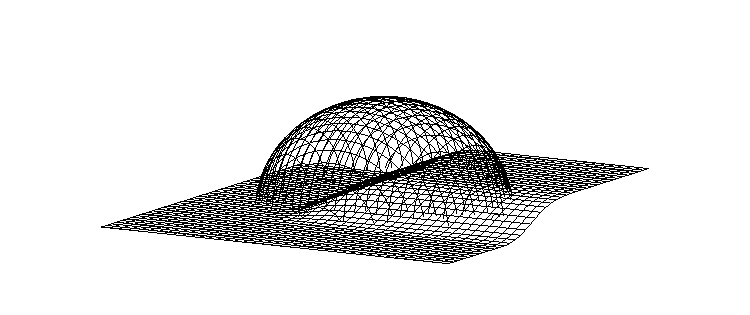
\includegraphics[height=120pt,trim=10 10 10 40,clip]{figures/surface.pdf}
  \caption{Boundary domain for the computation.}
  \label{fig:boundary_domain}
\end{figure*}

Consider a volume large enough to enclose the entire ground region that moves as a result of an underground explosion but small enough so that meterological effects can be neglected. In this volume
\[
\Big(\nabla^2+k^2\Big)P({\bf x},\omega)=0.
\]
Here $k=\frac{2\pi f}{c}$, where $f$ is angular frequency and $c$ is the speed of sound, is the wavenumber. If $B$ is the boundary of this volume then by the Kirchoff-Helmholtz integral formula \cite{morse1968theoretical}
\begin{equation}\label{eq:kirk_helm}
P({\bf x})
=
\int_{B} \bigg[
\Big({\bf \hat n}\cdot\nabla_{\bf y} G({\bf x},{\bf y})\Big)P({\bf y})
+
i\omega\rho G({\bf x},{\bf y}){\bf \hat n}\cdot{\bf v}({\bf y})
\bigg]\, d\sigma({\bf y}).
\end{equation}
for ${\bf x}$ not on the surface $B$. On the surface, for ${\bf x}\in B$, the overpressure satisfies 
\begin{equation}\label{eq:kirk_helm_P_on_surface}
c({\bf x})P({\bf x})
=
\int_{B} \bigg[
\Big({\bf \hat n}\cdot\nabla_{\bf y} G({\bf x},{\bf y})\Big)P({\bf y})
+
i\omega\rho G({\bf x},{\bf y}){\bf \hat n}\cdot{\bf v}({\bf y})
\bigg]\, d\sigma({\bf y})
\end{equation}
where $c({\bf x})$ is $\frac{1}{4\pi}$ times the solid angle ({\color{red} using a Greens' function is normalized to yield a delta function rather than a delta function over $4\pi$}) subtended by the computational volume at ${\bf x}$. 

Consider a sphere, $S$, of radius $R$ centered at the spot on the ground directly above the explosion. Choose the computational volume to be the intersection of the sphere with the region above the ground surface. Then $B=G\cup D$ where $G$ is the ground surface contained in $S$ and $D$ is the part of $S$ above the ground surface. Choosing the Green's function to have Dirichlet boundary conditions on $S$ one has
\begin{equation}\label{eq:kirk_helm_domain_dir_sphere}
\begin{aligned}
c({\bf x})P({\bf x})
=&
\int_{G} \bigg[
\Big({\bf \hat n}\cdot\nabla_{\bf y} G({\bf x},{\bf y})\Big)P({\bf y})
+
i\omega\rho G({\bf x},{\bf y}){\bf \hat n}\cdot{\bf v}({\bf y})
\bigg]\, d\sigma({\bf y})\\
&+
\int_{D} 
\Big({\bf \hat n}\cdot\nabla_{\bf y} G({\bf x},{\bf y})\Big)P({\bf y})
\, d\sigma({\bf y}).
\end{aligned}
\end{equation}
On $D$ one can use spherical coordinates $r,\theta,\phi$ and one then has $d\sigma=R^2\sin\theta\, d\theta d\phi$. On $G$, let $z=h(x,y)$ be the height of the ground, measured from the ground point directly above the explosion. Then one has 
\begin{equation}\label{eq:gnd_surface_element}
d\sigma=\sqrt{1+(\frac{\partial h}{\partial x})^2+(\frac{\partial h}{\partial y})^2\,}\, dx\, dy
\end{equation}
Note that ${\bf x}$ is inside the volume considered, and approaches the surface from the inside. In particular $\|{\bf x}\|\le R$. 

The surface velocity ${\bf v}$ is the source of the acoustic excitation in this problem. The principle of solution is to treat the above integral equation as a linear equation for the pressure $P$ on $B$ and solve for $P$. \cite{schenck1968improved,bai2013acoustic} This will be accomplished by using a version of the Galerkin method to approximate the integral equation with a linear system and then solve the linear system using a straightforward LU algorithm. Some subtleties arise in taking the limit as ${\bf x}$ approaches the surface $B$ and from singluar behavior of the Green's function at frequencies corresponding to resonances in a sphere with pressure release boundary conditions on its surface. This leads to spurious zero modes (modes with eigenvalue zero) in the resulting linear system. These subtleties are dealt with in the literature where they are called the ``nonuniqueness problem''. \cite{schenck1968improved} 

\subsection{The Green's Function:}\label{subsec:greens_func}

We construct the Green's function in sperical coordinates \cite{williams1999fourier}
\[
G(r_{\bf x},\theta_{\bf x},\phi_{\bf x},r_{\bf y},\theta_{\bf y},\phi_{\bf y})
=
\sum_{l,m}Y_{l,m}(\theta_{\bf x},\phi_{\bf x})Y_{l,m}^*(\theta_{\bf y},\phi_{\bf y})g_l(r_{\bf x},r_{\bf y})
\]
where 
\[
\Big(\secparderiv r + \frac{2}{r}\parderiv r - \frac{l(l+1)}{r^2} +k^2\Big)g_l(r,r^\prime)
=\frac{\delta(r-r^\prime)}{rr^\prime}
\]
and $k=\frac{\omega}{c}$. The radial component, $g_l(r,r^\prime)$, can be constructed out of spherical Bessel functions $j_l$ and $y_l$: 
\[
g_l(r,r^\prime)=kj_l(kr_<)\Big(y_l(kr_>)-\frac{y_l(kR)}{j_l(kR)}j_l(kr_>)\Big)
\]
where $r_<=\text{min}\{r,r^\prime\}$,  $r_>=\text{max}\{r,r^\prime\}$. 

Use can be made of the summation formula (see http://dlmf.nist.gov)
\[
\sum_{m=-l}^lY_{l,m}(\theta_{\bf x},\phi_{\bf x})Y_{l,m}^*(\theta_{\bf y},\phi_{\bf y})
=
\frac{2l+1}{4\pi}P_l\big(\cos\Omega(\theta_{\bf x},\phi_{\bf x},\theta_{\bf y},\phi_{\bf y})\big),
\]
where $P_l$ is the Legendre polynomial and $\Omega(\theta_{\bf x},\phi_{\bf x},\theta_{\bf y},\phi_{\bf y})$ is the angle between the vectors ${\bf x}$ and ${\bf y}$. Note that 
\[
\cos\Omega(\theta_{\bf x},\phi_{\bf x},\theta_{\bf y},\phi_{\bf y})=\cos\theta_{\bf x}\cos\theta_{\bf y}+\sin\theta_{\bf x}\sin\theta_{\bf y}\cos(\phi_{\bf x}-\phi_{\bf y}). 
\]
Substituting in one finds
\begin{equation}\label{eq:greens_function}
G(r_{\bf x},\theta_{\bf x},\phi_{\bf x},r_{\bf y},\theta_{\bf y},\phi_{\bf y})
=
\sum_{l=0}^\infty\frac{2l+1}{4\pi}P_l\big(\cos\Omega(\theta_{\bf x},\phi_{\bf x},\theta_{\bf y},\phi_{\bf y})\big)
kj_l(kr_<)\Big(y_l(kr_>)-\frac{y_l(kR)}{j_l(kR)}j_l(kr_>)\Big).
\end{equation}

The radial Green's function $g_l$ is singlular at frequencies for which 
\[
j_l(kR)=j_l(\frac{2\pi fR}{c})=0.
\]
The smallest zero of a spherical Bessel function is that of $j_0(x)$ at $x=\pi$ so that, for $c=340\text{ m/s}$ and $R$ in the range of hundreds of meters the lowest such frequency is around 1 Hz. At these frequencies one finds zero modes in the resulting linear system for $P$. A method (known in the literature as the CHIEF method) for handling the associated indeterminacy. Initially the code will be tested at frequencies where this is not an issue. The implementation of the CHIEF (or some other) method will be done at some later point. 

\subsection{The Normal Derivatives of the Greens' Function}

Note that, since $r_{\bf y}=R$ and $r_{\bf x}<R$ on $D$, 
\begin{align*}
{\bf \hat n}\cdot&\nabla_{\bf y} G({\bf x},{\bf y})\big|_{{\bf y}\in D}=\frac{\partial}{\partial r_{\bf y}} G({\bf x},{\bf y})\big|_{r_{\bf y}=R}
\\
&=\sum_l\frac{2l+1}{4\pi}P_l\big(\cos\Omega\big)\frac{\partial}{\partial r_{\bf y}} g_l(r_{\bf x},r_{\bf y})\big|_{r_{\bf y}=R}
\\
&=
\sum_l\frac{2l+1}{4\pi}P_l\big(\cos\Omega\big)
k^2\frac{j_l(kr_{\bf x})}{j_l(kR)}\Big(j_l(kR)y_l^\prime(kR)-j_l^\prime(kR)y_l(kR)\Big)
\\
&=
\sum_l\frac{2l+1}{4\pi}P_l\big(\cos\Omega\big)\frac{j_l(kr_{\bf x})}{R^2j_l(kR)}
\end{align*}
for ${\bf y}\in D$.

To compute the normal derivative on the ground surface $G$ one needs a parameterization of the surface. Recall that $z=h(x,y)$ is the height of the ground, measured from the ground point directly above the explosion. Then the unit normal to the ground surface is given by 
\[
{\bf \hat n}
=
\frac{1}{\sqrt{1+(\frac{\partial h}{\partial x})^2+(\frac{\partial h}{\partial y})^2}}
\begin{pmatrix}-\frac{\partial h}{\partial x}\\-\frac{\partial h}{\partial y}\\1\end{pmatrix}
\]
and
\[
{\bf \hat n}\cdot\nabla
=
\frac{1}{\sqrt{1+(\frac{\partial h}{\partial x})^2+(\frac{\partial h}{\partial y})^2}}
\Big(
-\frac{\partial h}{\partial x}\frac{\partial}{\partial x}-\frac{\partial h}{\partial y}\frac{\partial}{\partial y}
+\frac{\partial}{\partial z}
\Big).
\]
Transforming to spherical coordinates we use
\[
\parderiv x
=
\sin\theta\cos\phi\parderiv r
+
\frac{1}{ r}\cos\theta\cos\phi\parderiv \theta
-
\frac{\sin\phi}{ r\sin\theta}\parderiv \phi,
\]
\[
\parderiv y
=
\sin\theta\sin\phi\parderiv r
+
\frac{1}{ r}\cos\theta\sin\phi\parderiv \theta
+
\frac{\cos\phi}{ r\sin\theta}\parderiv \phi
\]
and
\[
\parderiv z
=
\cos\theta\parderiv r
-\frac{1}{ r}\sin\theta\parderiv \theta
\]
so that 
\begin{align*}
{\bf \hat n}\cdot\nabla
=
\frac{1}{\sqrt{1+(\frac{\partial h}{\partial x})^2+(\frac{\partial h}{\partial y})^2}}
\bigg[&
\Big(\cos\theta-\frac{\partial h}{\partial x}\sin\theta\cos\phi
-\frac{\partial h}{\partial y}\sin\theta\sin\phi\Big)\frac{\partial}{\partial r}\\
&-
\frac{1}{r}\Big(\sin\theta+\frac{\partial h}{\partial x}\cos\theta\cos\phi
+\frac{\partial h}{\partial y}\cos\theta\sin\phi\Big)\frac{\partial}{\partial \theta}\\
&+
\frac{1}{r}\Big(\frac{\partial h}{\partial x}\frac{\sin\phi}{ r\sin\theta}
-\frac{\partial h}{\partial y}\frac{\cos\phi}{ r\sin\theta}\Big)\frac{\partial}{\partial \phi}
\bigg].
\end{align*}
For ${\bf y}\in G$ on then has, with $G$ specified by $y_3=h(y_1,y_2)$, 
\begin{align*}
{\bf \hat n}\cdot\nabla_{\bf y} G({\bf x},{\bf y})
=&
\frac{1}{\sqrt{1+(\frac{\partial h}{\partial y_1})^2+(\frac{\partial h}{\partial y_2})^2}}
\sum_{l=0}^\infty\frac{2l+1}{4\pi}\\
&\bigg[
\Big(\cos\theta_{\bf y}-\frac{\partial h}{\partial y_1}\sin\theta_{\bf y}\cos\phi_{\bf y}
-\frac{\partial h}{\partial y_2}\sin\theta_{\bf y}\sin\phi_{\bf y}\Big)\frac{\partial}{\partial r_{\bf y}}\\
&-
\frac{1}{r_{\bf y}}\Big(\sin\theta_{\bf y}+\frac{\partial h}{\partial y_1}\cos\theta_{\bf y}\cos\phi_{\bf y}
+\frac{\partial h}{\partial y_2}\cos\theta_{\bf y}\sin\phi_{\bf y}\Big)\frac{\partial}{\partial \theta_{\bf y}}\\
&+
\frac{1}{r_{\bf y}}\Big(\frac{\partial h}{\partial y_1}\frac{\sin\phi_{\bf y}}{ r\sin\theta_{\bf y}}
-\frac{\partial h}{\partial y_2}\frac{\cos\phi_{\bf y}}{ r\sin\theta_{\bf y}}\Big)\frac{\partial}{\partial \phi_{\bf y}}
\bigg]P_l(\cos\Omega)g_l(r_{\bf x},r_{\bf y}).
\end{align*}
One has 
\[
\frac{\partial}{\partial r_{\bf y}}g_l(r_{\bf x},r_{\bf y})
=
k^2\begin{cases}
j_l(kr_{\bf x})\Big(y_l^\prime(kr_{\bf y})-\frac{y_l(kR)}{j_l(kR)}j_l^\prime(kr_{\bf y})\Big) & \text{if } r_{\bf x}<r_{\bf y}\\
j_l^\prime(kr_{\bf y})\Big(y_l(kr_{\bf x})-\frac{y_l(kR)}{j_l(kR)}j_l(kr_{\bf x})\Big) & \text{if } r_{\bf y}<r_{\bf x}
\end{cases}.
\]
Using the relation for the derivatives of the spherical Bessel functions, 
\[
f_l^\prime(x)=-f_{l+1}(x)+\frac{l}{x}f_l(x),
\]
where $f_l$ is either $j_l$ or $y_l$, one finds 
\[
\frac{\partial}{\partial r_{\bf y}}g_l(r_{\bf x},r_{\bf y})
=
k^2\begin{cases}
j_l(kr_{\bf x})\Big(-y_{l+1}(kr_{\bf y})+\frac{l}{kr_{\bf y}}y_l(kr_{\bf y})-\frac{y_l(kR)}{j_l(kR)}\big(-j_{l+1}(kr_{\bf y})+\frac{l}{kr_{\bf y}}j_l(kr_{\bf y})\big)\Big) & \text{if } r_{\bf x}<r_{\bf y}\\
\Big(-j_{l+1}(kr_{\bf y})+\frac{l}{kr_{\bf y}}j_l(kr_{\bf y})\Big)
\Big(y_l(kr_{\bf x})-\frac{y_l(kR)}{j_l(kR)}j_l(kr_{\bf x})\Big) & \text{if } r_{\bf y}<r_{\bf x}
\end{cases}.
\]
and using 
\[
(1-x^2)\frac{dP_l}{dx}={-(l+1)P_{l+1}(x)+(l+1)xP_l(x)}
\]
one finds
\[
\frac{\partial}{\partial \theta_{\bf y}}P_l(\cos\Omega)
=
\frac{1}{\sin^2\Omega}\Big({-(l+1)P_{l+1}(\cos\Omega)+(l+1)\cos\Omega P_l(\cos\Omega)}\Big)
\frac{\partial\Omega}{\partial \theta_{\bf y}}
\]
and
\[
\frac{\partial}{\partial \phi_{\bf y}}P_l(\cos\Omega)
=
\frac{1}{\sin^2\Omega}\Big({-(l+1)P_{l+1}(\cos\Omega)+(l+1)\cos\Omega P_l(\cos\Omega)}\Big)
\frac{\partial\Omega}{\partial \phi_{\bf y}}
\]


\newpage



\section{Reduction to a Discrete Problem:}\label{sec:discretization}

The integrals are rendered discrete using a finite element approximation. Perhaps the simplest formulation of the finite elements that provides continuous approximations to the integrands are linear interpolation funcitons on triangular elements. These are defined by a specification of vertices $(x_j,x_k)$ and of the sides defining the enclosed triangles. The interpolating functions $\psi_{jk}$ are ..... {\color{red} need to beef up this introductory section}

\subsection{The Overpressure on the Ground Surface}\label{subsec:gnd_surface}

\vspace*{5pt}

Consider first 
\begin{align*}
{\cal P}_G({\bf x})&=\int_{G}{\bf \hat n}\cdot\nabla_{\bf y} G({\bf x},{\bf y})P({\bf y}) \, d\sigma({\bf y})\\
&=
\int_{G}
P({\bf y}){\bf \hat n}\cdot\nabla_{\bf y} G({\bf x},{\bf y})
\sqrt{1+(\frac{\partial h}{\partial y_1})^2+(\frac{\partial h}{\partial y_2})^2\,} \, dy_1\, dy_2\\
&=
\int_0^R\int_0^{2\pi} P\big(r\cos\theta,r\sin\theta,h(r\cos\theta,r\sin\theta)\big){\cal G}({\bf x},r,\theta)\, rd\theta\, dr
\end{align*}
where
\[
{\cal G}({\bf x},r,\theta)
=
{\bf \hat n}\cdot\nabla_{\bf y} G({\bf x},{\bf y})
\sqrt{1+(\frac{\partial h}{\partial y_1})^2+(\frac{\partial h}{\partial y_2})^2\,}\, \bigg|_{y_1=r\cos\theta,y_2=r\sin\theta}.
\]

\begin{figure*}[h]
  \centering
  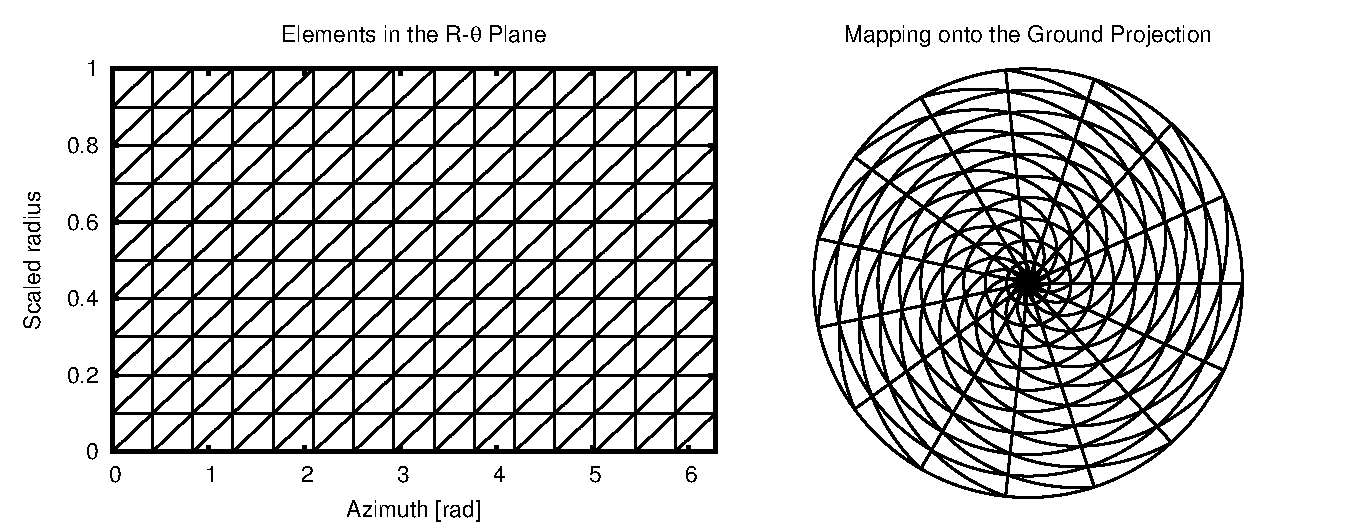
\includegraphics[height=160pt]{figures/ground_elements.pdf}
  \caption{Schematic for a boundary element discretization for the ground surface.}
  \label{fig:ground_elements}
\end{figure*}

\begin{figure*}[h]
  \centering
  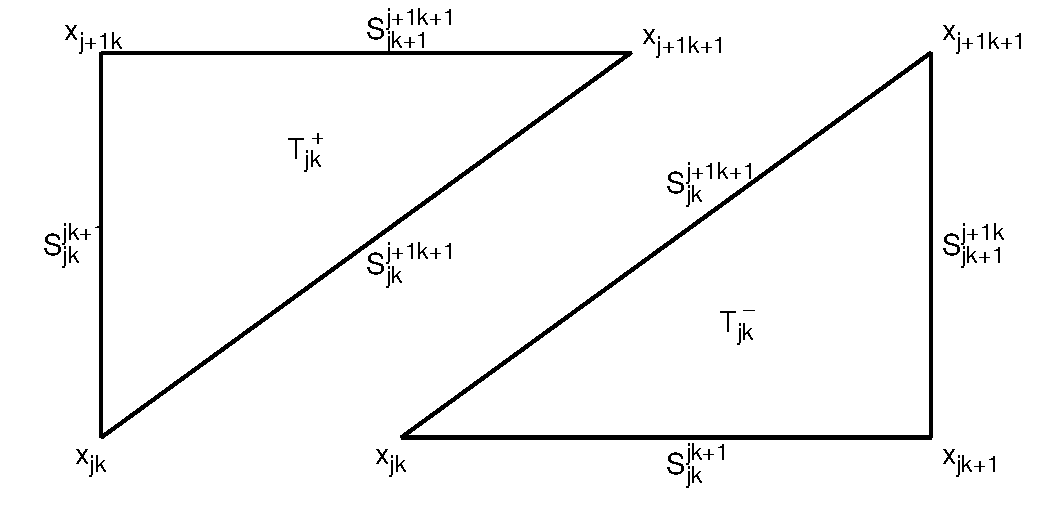
\includegraphics[height=130pt]{figures/ground_triangles.pdf}
  \caption{Two types of triangular elements for the ground surface.}
  \label{fig:ground_triangles}
\end{figure*}

One possible scheme for the ground surface is shown above in Fig.\, \ref{fig:ground_elements}. Here the vertices are given by 
\[
x_{jk}=(j\frac{R}{N},k\frac{2\pi}{M})
\]
with $j\in\{0,1,2,\dots,N\}$, $k\in\{0,1,2,\dots,M\}$. The sides are of three types: 
\[
S_{jk}^{j+1 k}\ \text{from}\ x_{jk}\ \text{to}\ x_{j+1 k}
\]
\[
S_{jk}^{j k+1}\ \text{from}\ x_{jk}\ \text{to}\ x_{j k+1}
\]
and
\[
S_{jk}^{j+1 k+1}\ \text{from}\ x_{jk}\ \text{to}\ x_{j+1 k+1}.
\]
There are two types of triangles, $T^{\pm}_{jk}$, one with vertices $x_{jk},x_{j+1 k}, x_{j+1 k+1}$ the other $x_{jk},x_{j k+1}, x_{j+1 k+1}$. The two types of triangle are shown in Fig.\, \ref{fig:ground_triangles}. 

The overpressure is approximated by interpolating from values at the vertices, 
\[
{\cal P}_G({\bf x})
\approx
\sum_{j=1}^N\sum_{k=1}^M {\cal P}_{j,k}
\int\int{\cal G}({\bf x},r,\theta)\psi^{G}_{jk}(r,\theta)\, r\, d\theta\, dr, 
\]
where the values ${\cal P}_{j,k}$ are to be determined. Note that, to enforce periodicity in $\theta$, ${\cal P}_{j,0}={\cal P}_{j,M}$. The interpolating functions, $\psi^{G}_{jk}(r,\theta)$, are compactly supported, piecewise linear functions constructed as follows. 

\begin{figure*}[h]
  \centering
  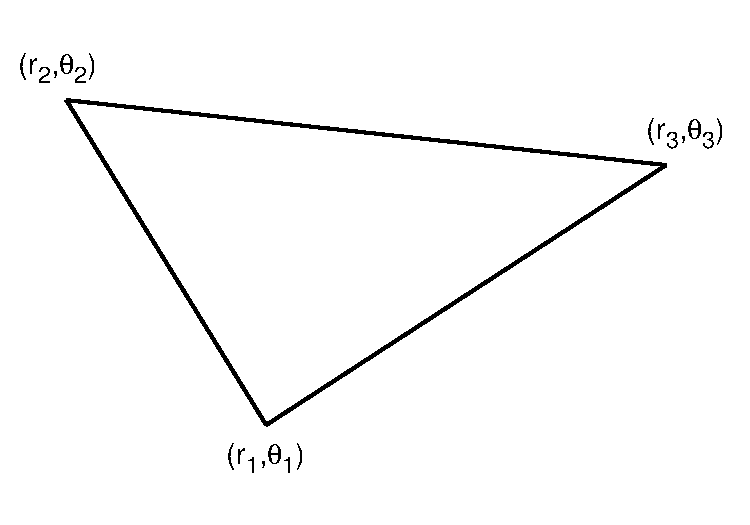
\includegraphics[height=130pt]{figures/gen_triangle.pdf}
  \caption{A generic triangular element.}
  \label{fig:gen_triangle}
\end{figure*}

\noindent For each triangle, $T^{\pm}_{jk}$, introduce three functions $u_{jk}^{\pm;m}(r,\theta)$, one for each vertex $m=(r_1,\theta_1),(r_2,\theta_2),(r_3,\theta_3)$, which are $0$ outside $T^{\pm}_{jk}$, are given by  
\[
u_{jk}^{\pm;m}(r,\theta)=a_{jk}^{\pm;m}+b_{jk}^{\pm;m}r+c_{jk}^{\pm;m}\theta
\] 
in $T^{\pm}_{jk}$ and for which the coefficents $a_{jk}^{\pm;m}$, $b_{jk}^{\pm;m}$ and $c_{jk}^{\pm;m}$ are determined by the conditions that $u_{jk}^{\pm;m}$ are equal to $1$ at the vertex $m$ and $0$ at the other vertices. General formulae can be developed as follows. Consider the generic element shown in Fig.\, \ref{fig:gen_triangle}. The the interpolation functions $u^m$ satisfy 
\[
u^m(n)=\delta_{mn}
\]
for vertices $m,n$. This leads to the equations 
\[
\begin{pmatrix}
1 & r_1 & \theta_1 \\
1 & r_2 & \theta_2 \\
1 & r_3 & \theta_3 
\end{pmatrix}
\begin{pmatrix}
a^m\\b^m\\c^m
\end{pmatrix}
=
\begin{pmatrix}
\delta_{mn_1}\\\delta_{mn_2}\\\delta_{mn_3}
\end{pmatrix}.
\]
These are straightforward to solve. 

\begin{figure}[h]
  \centering
  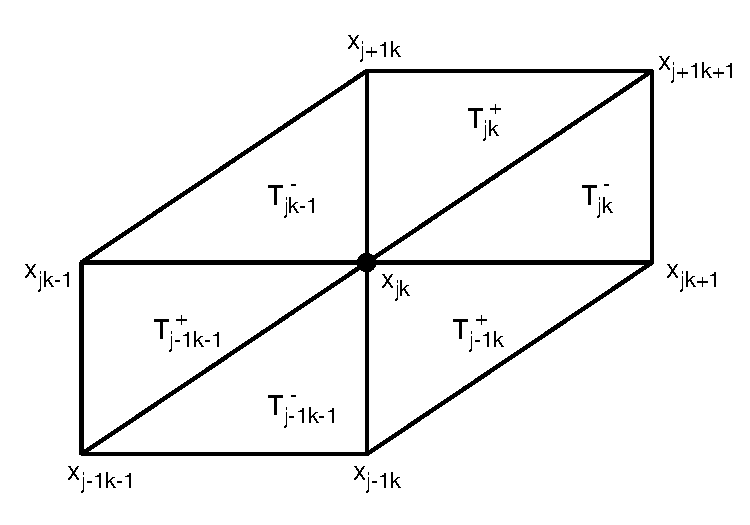
\includegraphics[height=130pt]{figures/ground_triangles_interp.pdf}
  \caption{The six triangles associated with interpolation at the vertex $x_{jk}$.}
  \label{fig:int_triangles}
\end{figure}

Given the $u_{jk}^{\pm;m}(r,\theta)$, for vertices in the interior of the ground disk, for $1\le j \le N-1$ and  $1\le k \le M-1$, one has
\[
\psi^{G}_{jk}(r,\theta)
=
u_{jk}^{+;x_{jk}}(r,\theta)+u_{jk}^{-;x_{jk}}(r,\theta)
+
u_{j-1k}^{+;x_{jk}}(r,\theta)+u_{jk-1}^{-;x_{jk}}(r,\theta)
+
u_{j-1k-1}^{+;x_{jk}}(r,\theta)+u_{j-1k-1}^{-;x_{jk}}(r,\theta).
\]
To enforce periodicity field values at a fixed radius $r$ (or $j$) for $\theta=0$ (equivalently $k=0$) are the same as the field values at that radius for $\theta=2\pi$ (equivalently $k=M$). Thus, for $1\le j \le N-1$ 
\[
\psi^{G}_{j0}(r,\theta)
=
u_{j0}^{+;x_{j0}}(r,\theta)+u_{j0}^{-;x_{j0}}(r,\theta)+u_{j-10}^{+;x_{j0}}(r,\theta)
+
u_{jM-1}^{-;x_{jM}}(r,\theta)+u_{j-1M-1}^{-;x_{jM}}(r,\theta)+u_{j-1M-1}^{+;x_{jM}}(r,\theta).
\]
At the central point, $r=0$ (equivalently $j=0$), there is only one physical vertex so all field values are the same. The interpolation about the central point requires a special notation. We will use $\psi^{G}_{00}$ defined by 
$$
\psi^{G}_{00}=
U_{00}^{+;x_{00}}(r,\theta)+u_{00}^{-;x_{00}}(r,\theta)+u_{0M}^{-;x_{0M}}
+
\sum_{k=1}^{M-1}\Big(u_{0k}^{+;x_{0k}}(r,\theta)+u_{0k}^{-;x_{0k}}(r,\theta)+u_{0k-1}^{-;x_{0k}}(r,\theta)\Big)
$$




\bigskip\bigskip

{\color{red} THESE FOLLOWING ARE WRONG: for $j=N$ the pressure is also interpolated on the sphere!!!}

......................................................................................................


for $1\le k \le M-1$, 
\[
\psi^{G}_{0k}(r,\theta)
=
u_{0k}^{+;x_{0k}}(r,\theta)+u_{0k}^{-;x_{0k}}(r,\theta)+u_{0k-1}^{-;x_{0k}}(r,\theta)
\]
and, to enforce periodicity, 

.................


and  
\[
\psi^{G}_{Nk}(r,\theta)
=
u_{N-1k-1}^{+;x_{Nk}}(r,\theta)+u_{N-1k-1}^{-;x_{Nk}}(r,\theta)+u_{N-1k-1}^{+;x_{Nk}}(r,\theta),
\]




\[
\psi^{G}_{00}(r,\theta)
=
u_{00}^{+;x_{00}}(r,\theta)+u_{00}^{-;x_{00}}(r,\theta)+u_{0M-1}^{-;x_{0M}}(r,\theta),
\]
and
\[
\psi^{G}_{N0}(r,\theta)
=
u_{N-10}^{+;x_{N0}}(r,\theta)+u_{N-1M-1}^{+;x_{NM}}(r,\theta)+u_{N-1M-1}^{-;x_{NM}}(r,\theta){\color{red} ++++++}
\]
{\color{red} \text{PLUS THE TRIANGLES ON THE SPHERICAL SECTION!!!!!!}}.

\vspace*{10pt}

\noindent{\bf The Velocity on the Ground Surface}

\vspace*{5pt}

Now consider the integral over the ground surface of the contribution from the normal surface velocity
\[
{\cal P}_V({\bf x})=i\omega\rho \int_{G} G({\bf x},{\bf y}){\bf \hat n}\cdot{\bf v}({\bf y})\, d\sigma({\bf y}).
\]
This integral can be discretized similarly, except that the values of the normal component of the surface velocity, ${\bf \hat n}\cdot{\bf v}$, are assumed to be known. In principle they have been measured. Ideally these measurements are used as nodal values in a triangularization, except that the accelerometer deployments for SPE 5 and 6 were not dense enough. As a consequence some model based interpolation must be used. {\color{Blue} \{This needs to be investigated. Need accelerometer data.\}} In any event, a triangularization for the ground surface, possibly the same as for the overpressure contribution, and associated interpolation functions $\psi^{V}_{jk}(r,\theta)$, again possibly but not necessarily the same as used for the overpressure, will lead to 
\[
{\cal P}_V({\bf x})
\approx 
i\omega\rho \sum_{jk} {\cal V}_{jk}
\int\int G({\bf x},r\cos\theta,r\sin\theta,h(r,\theta))\psi^{V}_{jk}(r,\theta)\, r\, d\theta\, dr
\]
where ${\cal V}$ are the (known) values of ${\bf \hat n}\cdot{\bf v}$ at the vertices. 

\vspace*{10pt}

\noindent{\bf The Overpressure on the Sphere Section}

\vspace*{5pt}

Now consider the integral over $D$. Recall that $D$ is the intersection of the sphere of radius $R$ with the space above the ground surface. Explicitly, 
\[
D=
\{(R\sin\theta\cos\phi,R\sin\theta\sin\phi,R\cos\theta)
\big|
\, 0\le\phi<2\pi, 0<\theta\le\pi,
R\cos\theta\ge h(R\sin\theta\cos\phi,R\sin\theta\sin\phi)\}.
\]
Let the solution to $R\cos\theta = h(R\sin\theta\cos\phi,R\sin\theta\sin\phi)$ be given by the curve $\theta=B(\phi)$. Given a form (analytic or otherwise) for $h(x,y)$, $B(\phi)$ can be obtained numerically for each $\phi$ in an array of azimuths. 

\begin{figure*}[h]
  \centering
  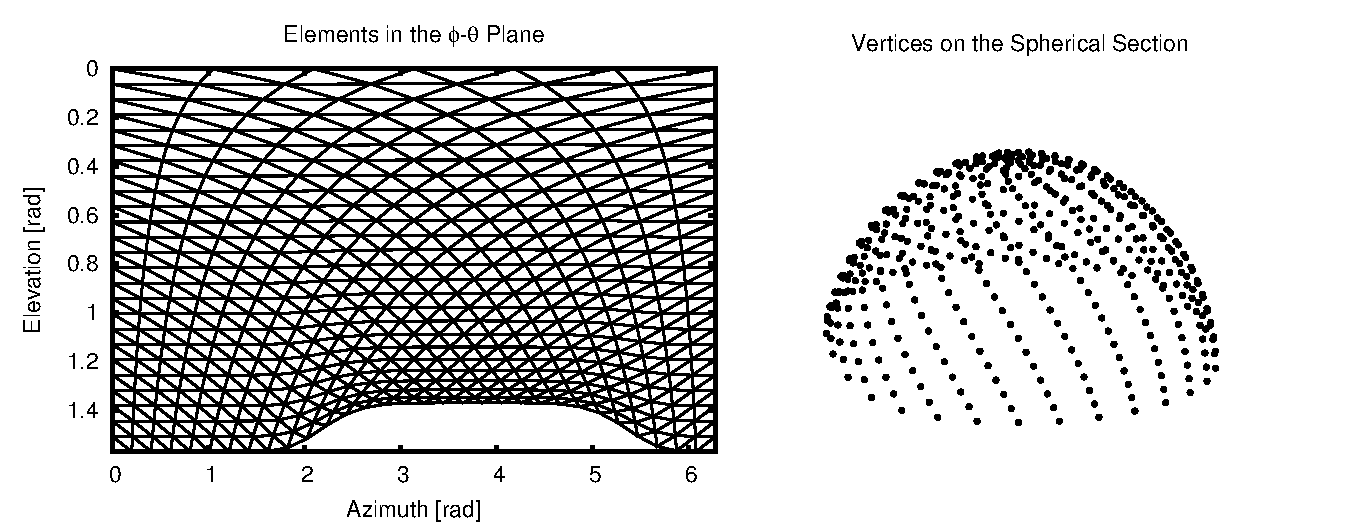
\includegraphics[height=160pt]{figures/sphere_section_elements.pdf}
  \caption{Schematic for a boundary element discretization for the surface of the spherical section for a simple model for $B(\phi)$.}
  \label{fig:spherical_section_elements}
\end{figure*}

One possible scheme for discretizing the spherical section, $D$, is to choose a grid of points in then $\phi - \theta$ plane given by the point $(0,0)$ and the points
\[
(\phi_j,\theta_k)=(j\Delta_{k,\phi},\alpha^{k-1}B(\phi_j)-k\Delta_\theta)
\]
where $0<\alpha<1$, allowing the grid to conform to the ground surface but to flatten out with increasing elevation, $\Delta_{k,\phi}<\Delta_{k+1,\phi}$, so that the number of azimuthal points decrease with increasing elevation. The point $(0,0)$ is added at the cap of the sphere. Triangles are then obtained by connecting grid points, which become the vertices of the triangles and interpolation functions are introduced as for the ground surface. In Fig.\,\ref{fig:spherical_section_elements} an example of such a triangularlization is shown. For purposes of illustration the form 
\[
B(\phi)=0.2e^{-(0.6*(\phi-1.2*\pi))^6}
\]
is assumed. The values $\Delta_k=\frac{\pi}{50}$, $\Delta_{k,\phi}=\frac{2\pi}{31-k}$ and $\alpha=0.8$ were used. Given a triangulaization with interpolation functions $\psi^{D}_{jk}(\theta,\phi)$ and introducing the notation 
\[
\Big({\bf \hat n}\cdot\nabla_{\bf y} G({\bf x},{\bf y})\Big)\Big|_D={\cal H}(\theta,\phi)
\]
one has 
\begin{align*}
{\cal P}_D({\bf x})
&=
\int_{D} 
\Big({\bf \hat n}\cdot\nabla_{\bf y} G({\bf x},{\bf y})\Big)P({\bf y})
\, d\sigma({\bf y})\\
&\approx
R^2\sum_{jk} {\cal P}_{jk}\int_0^\pi\int_0^{2\pi} {\cal H}(\theta,\phi)\psi^{D}_{jk}(\theta,\phi)\sin\theta\, d\theta d\phi
\end{align*}
where, again, periodicity in $\phi$ needs to be enforced. 


\newpage

{\color{Blue} 
\vspace*{15pt}

\noindent {\bf\large Left to do:}

\vspace*{10pt}

\begin{figure*}[h]
  \centering
  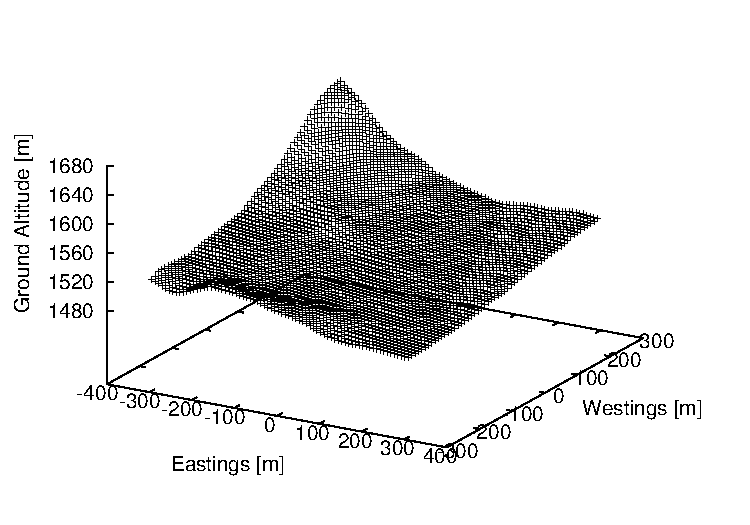
\includegraphics[height=200pt]{figures/SPE_ground_surface.pdf}
  \caption{{\color{Blue} Map of the ground surface at the SPE site.}}
\end{figure*}

\noindent {\bf\large Code development:}

\begin{itemize}
\item[] Algorithm development is close to being finished
  \begin{itemize}
  \item A toy (test) ground motion model needs to be developed
  \item The resulting linear algebra problem should be made as explicit as possible.
  \item Coding should begin 
    \begin{itemize}
    \item A toy model should be implemented in C/C++.
    \item The spurious zero mode issue needs to be investigated and addressed. 
    \end{itemize}
  \end{itemize}
\end{itemize}

\vspace*{10pt}

\noindent {\bf\large The SPE Shots:}

\vspace*{10pt}

\begin{itemize}
\item[] Ground topography at the site
  \begin{itemize}
  \item A surface map has been obtained with 10 meter resolution
  \item Bicubic splines to be used to interpolate. 
  \item Need to code up the $B(\phi)$ function determination.
  \end{itemize}
\end{itemize}

\begin{itemize}
\item[] Ground motion
  \begin{itemize}
  \item Accelerometer data is being obtained. 
  \item Need to settle on a data driven ground motion model. 
  \end{itemize}
\end{itemize}

}


\bibliographystyle{ieeetr}
\bibliography{boundary_element}

\end{document}